\section{Discussion}

\begin{figure}[ht]
    \centering

    \begin{subfigure}[b]{0.49\textwidth}
    \centering
    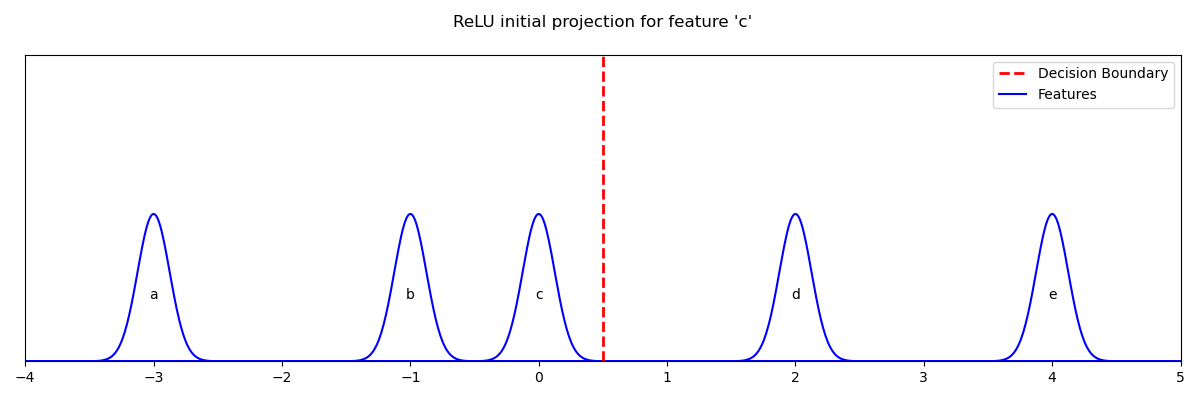
\includegraphics[width=\textwidth]{images/activation_demo_relu_pre}
    \caption{ReLU pre-activation projection}
    \label{fig:relu_pre}
    \end{subfigure}
    \hfill
    \begin{subfigure}[b]{0.49\textwidth}
    \centering
    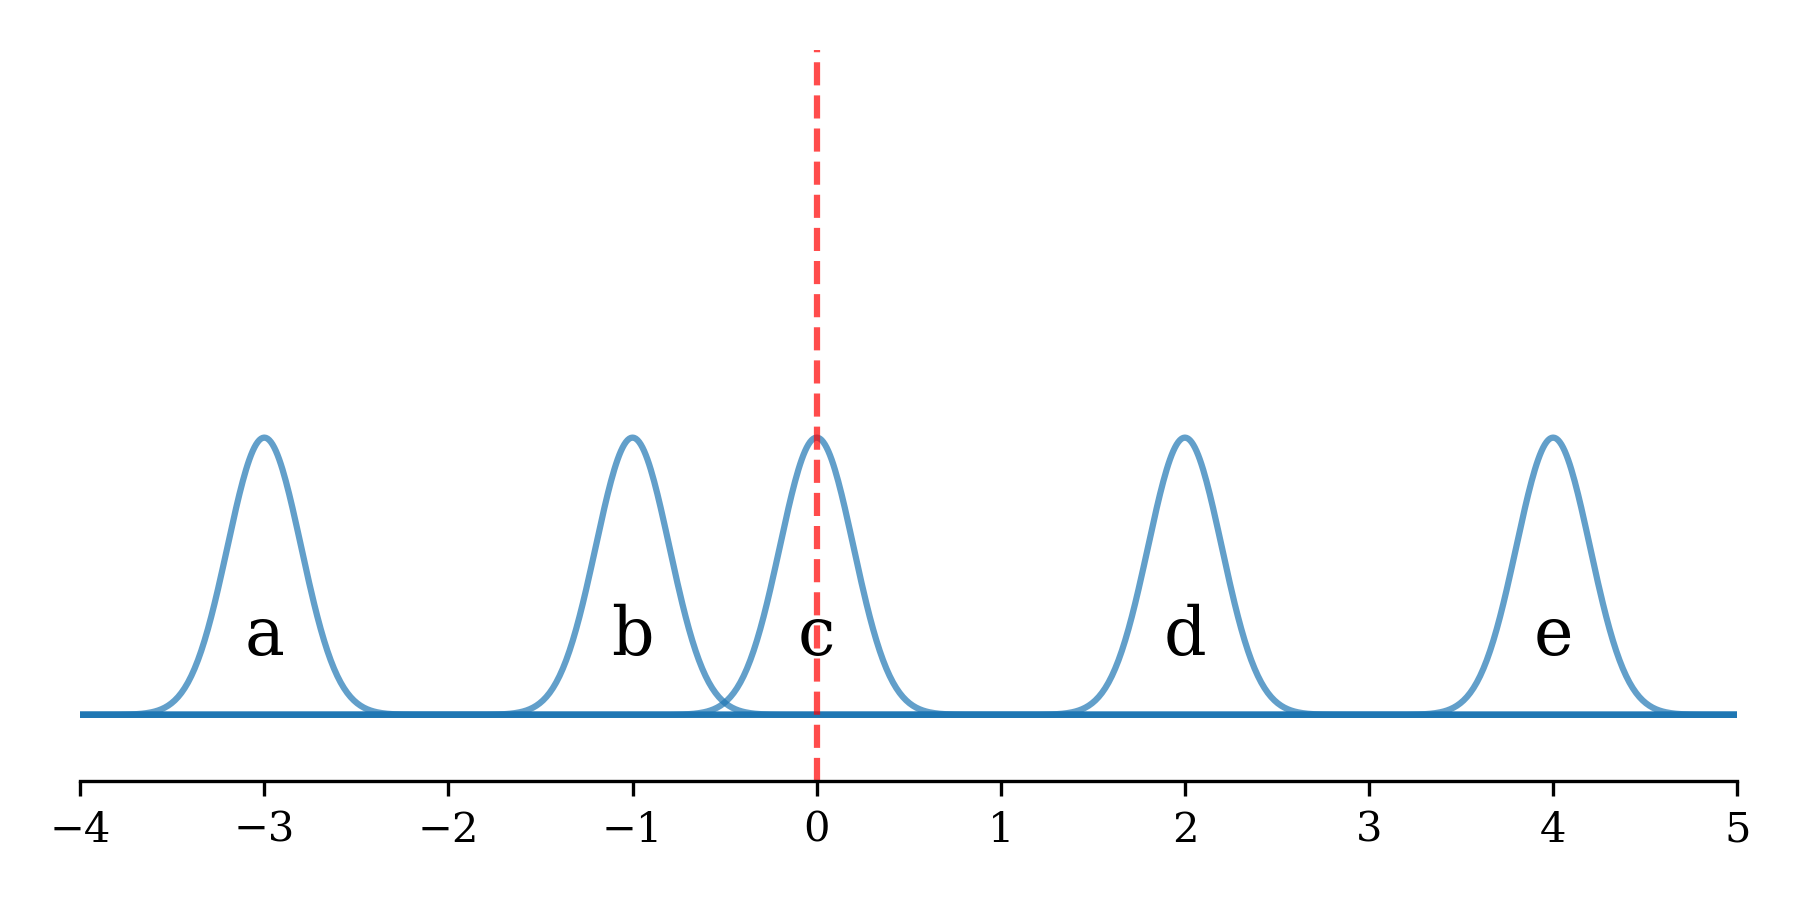
\includegraphics[width=\textwidth]{images/activation_demo_abs_pre}
    \caption{Abs pre-activation projection}
    \label{fig:abs_pre}
    \end{subfigure}

    \begin{subfigure}[b]{0.49\textwidth}
        \centering
        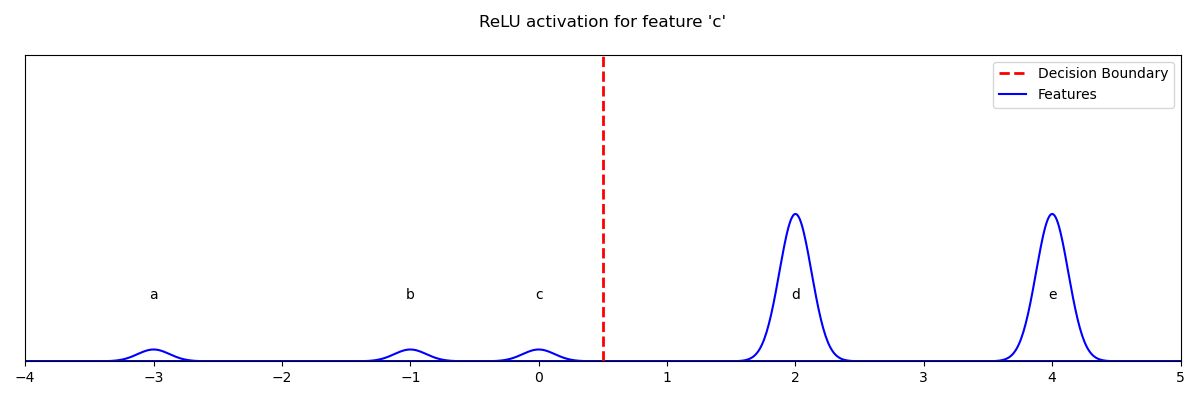
\includegraphics[width=\textwidth]{images/activation_demo_relu_post}
        \caption{ReLU post-activation response}
        \label{fig:relu_post}
    \end{subfigure}
    \hfill
    \begin{subfigure}[b]{0.49\textwidth}
        \centering
        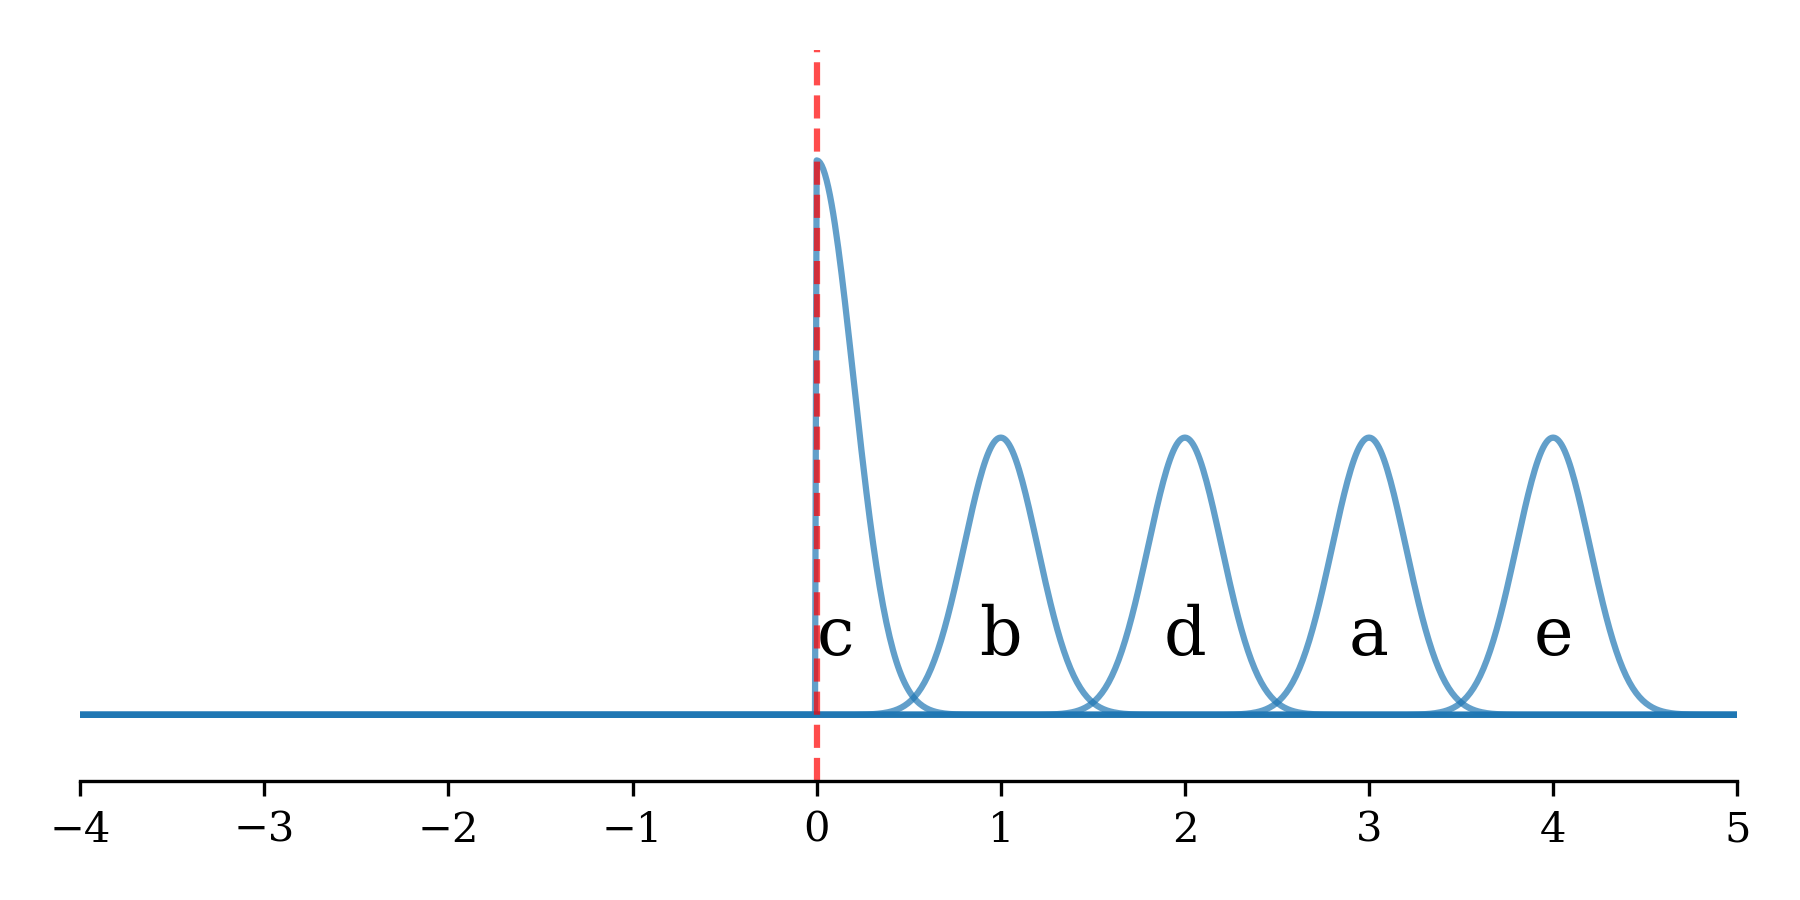
\includegraphics[width=\textwidth]{images/activation_demo_abs_post}
        \caption{Abs post-activation response}
        \label{fig:abs_post}
    \end{subfigure}

    \caption{This series of figures represents our theory on how linear nodes learn features with ReLU and Absolute Value activation functions. Each blue peak corresponds to a feature (a-e) in the hypothetical dataset, and the red dashed line denotes the decision boundary defined by the node. In the top row, the features are positioned according to their initial linear projections. The bottom row illustrates the transformed values after applying each activation function, highlighting the distinct ways that ReLU and Absolute Value modify feature space representations.}
    \label{fig:activation_demo}
\end{figure}

We explore how ReLU and Abs activations represent features within a distance metric interpretation. Figure~\ref{fig:activation_demo} illustrates the key differences in how these activation functions process information. In the pre-activation space (Figures~\ref{fig:relu_pre} and~\ref{fig:abs_pre}), both models can learn similar linear projections of input features. ReLU is driven to minimize the active feature $\left\{ c \right\}$ and ends up being positioned on the positive edge of the distribution. Abs positions the decision boundary through the mean, or possibly the median, of the data. After activation, ReLU sets all features on its dark side to the minimum possible distance: zero. Abs folds the space, moving all distributions on the negative side to the positive side. The ReLU activated node, selects for features $\left\{ a, b, c \right\}$. The folding operation of the Abs activated feature results in $\left\{ c \right\}$ being the sole feature with the smallest activation value.

\subsection{Offset Perturbations}

\begin{figure}[ht]
    \centering

    \begin{subfigure}[b]{0.49\textwidth}
        \centering
        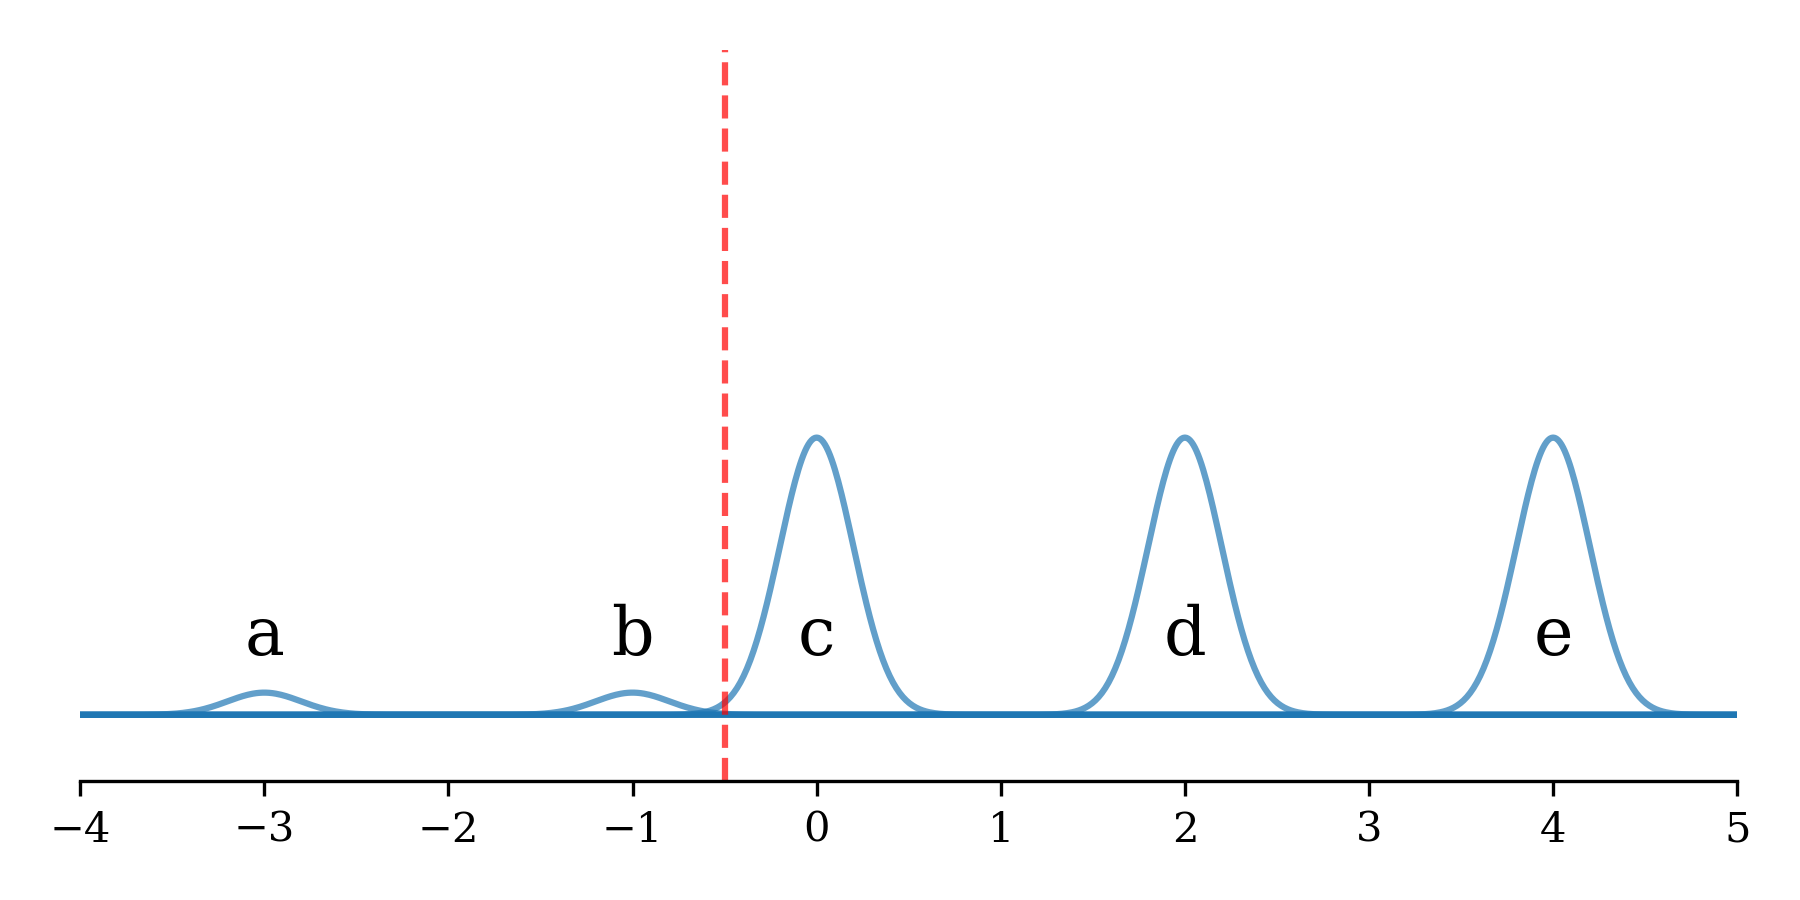
\includegraphics[width=\textwidth]{images/offset_relu_neg}
        \caption{ReLU Negative Offset}
        \label{fig:relu_offset_down}
    \end{subfigure}
    \hfill
    \begin{subfigure}[b]{0.49\textwidth}
        \centering
        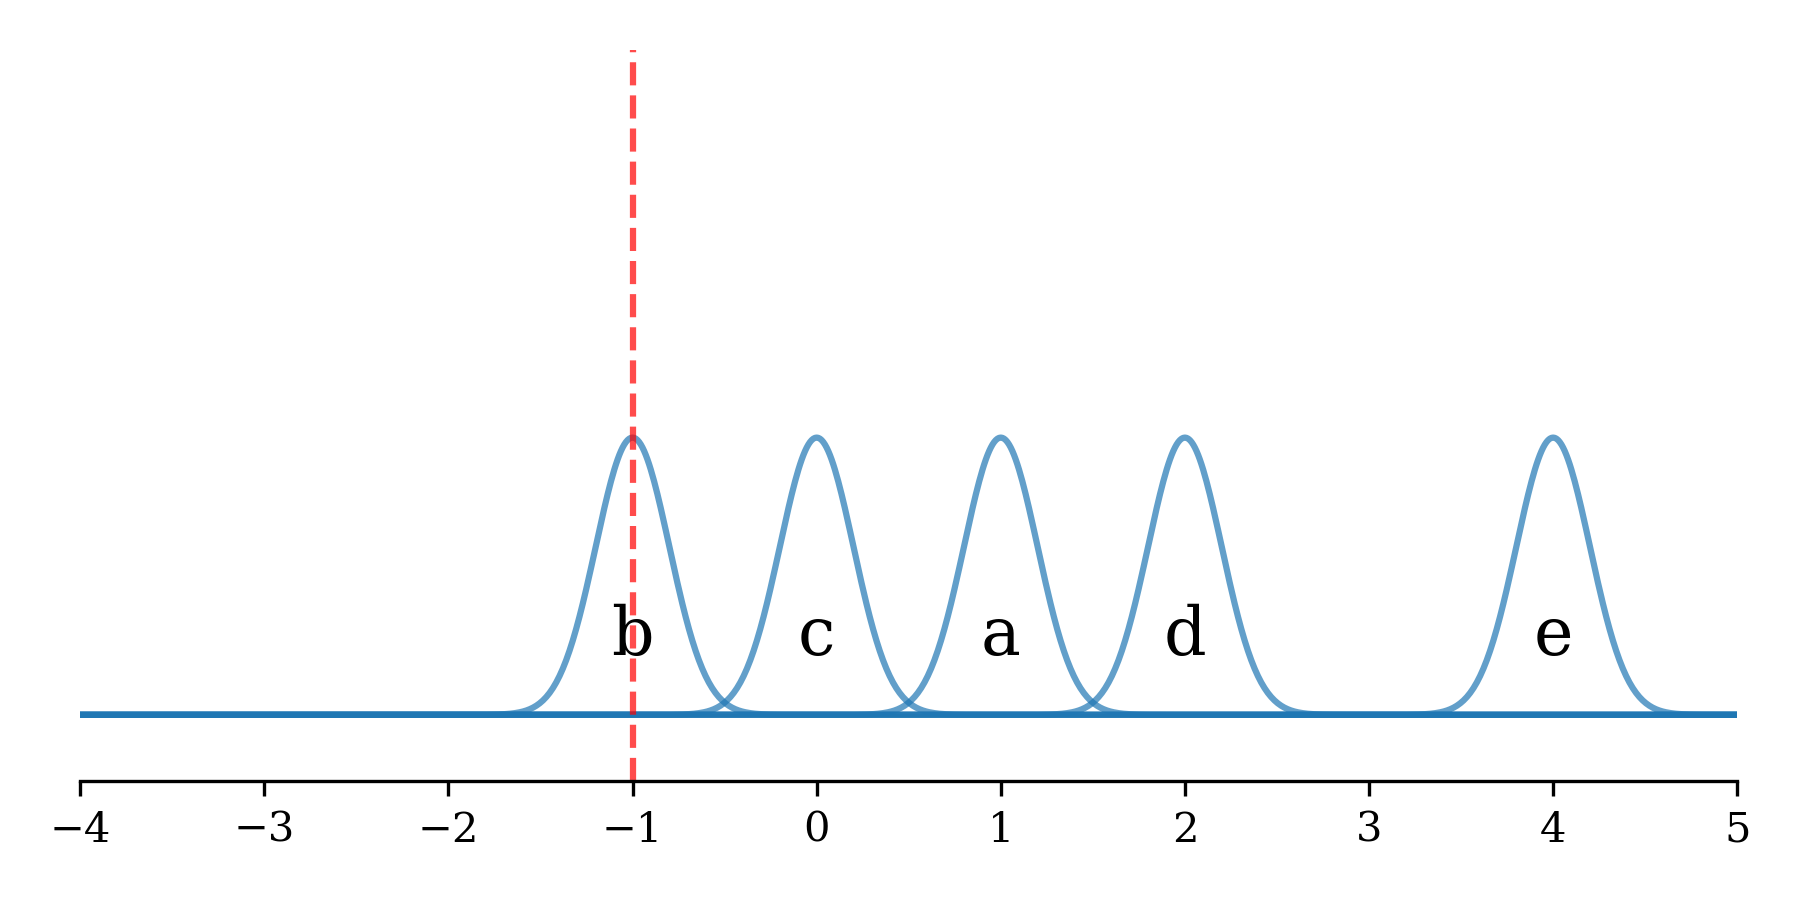
\includegraphics[width=\textwidth]{images/offset_abs_neg}
        \caption{Abs Negative Offset}
        \label{fig:abs_offset_down}
    \end{subfigure}

    \begin{subfigure}[b]{0.49\textwidth}
        \centering
        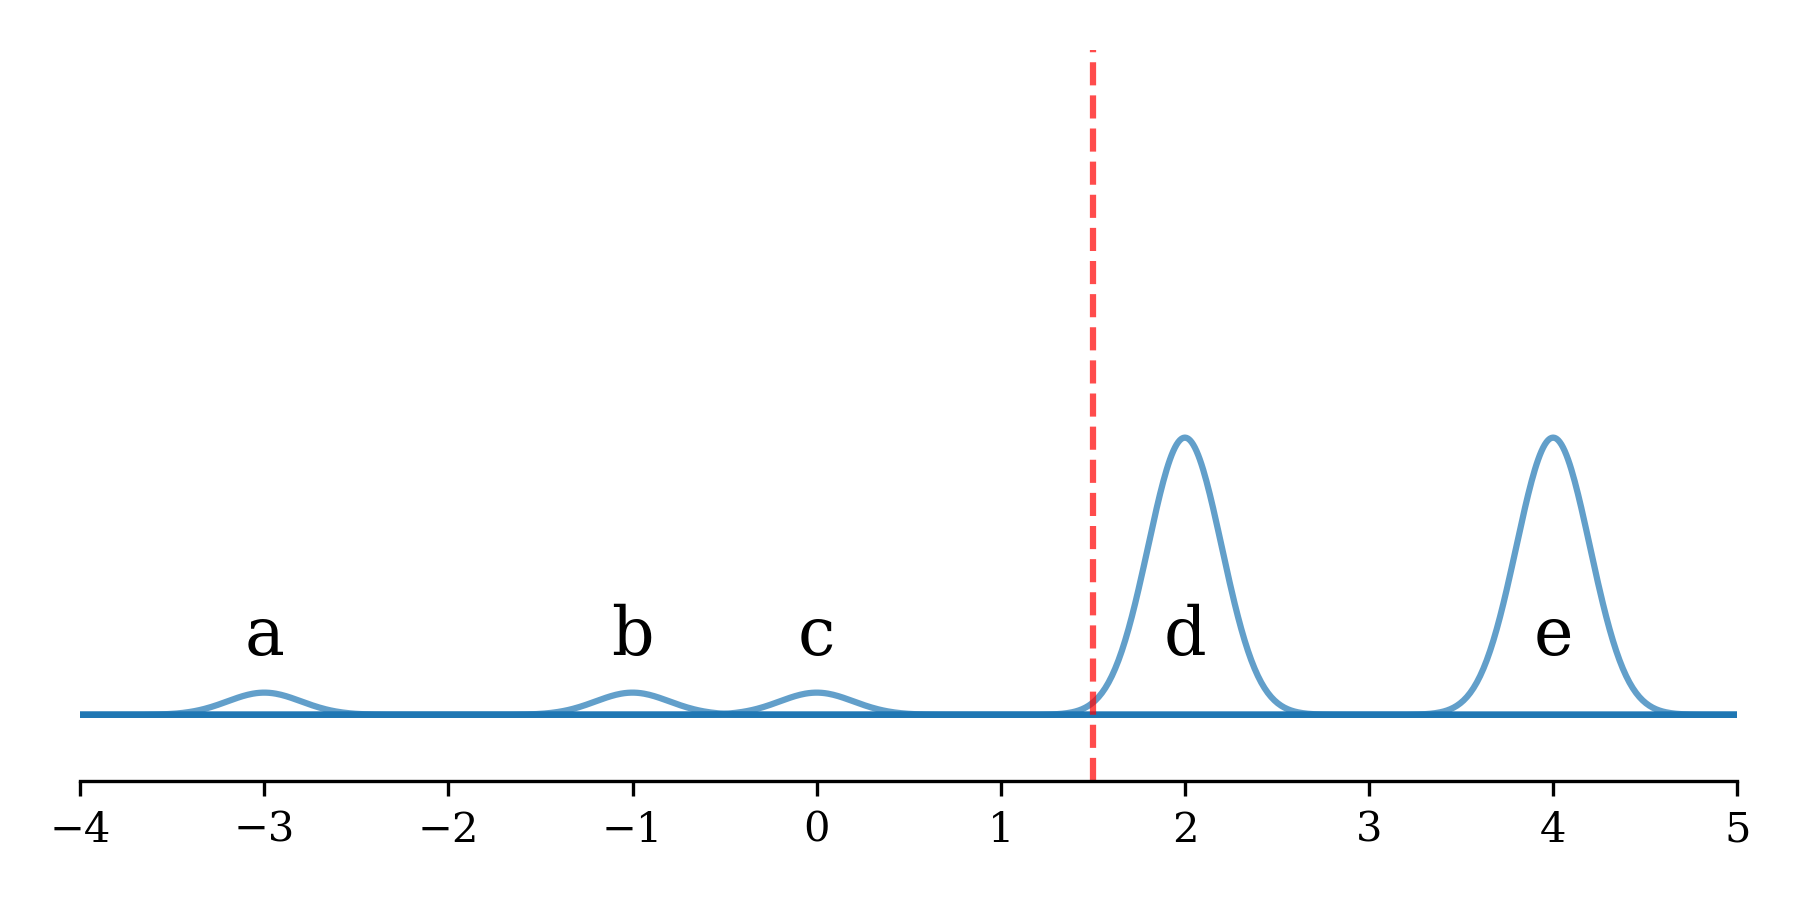
\includegraphics[width=\textwidth]{images/offset_relu_pos}
        \caption{ReLU Positive Offset}
        \label{fig:relu_offset_up}
    \end{subfigure}
    \hfill
    \begin{subfigure}[b]{0.49\textwidth}
        \centering
        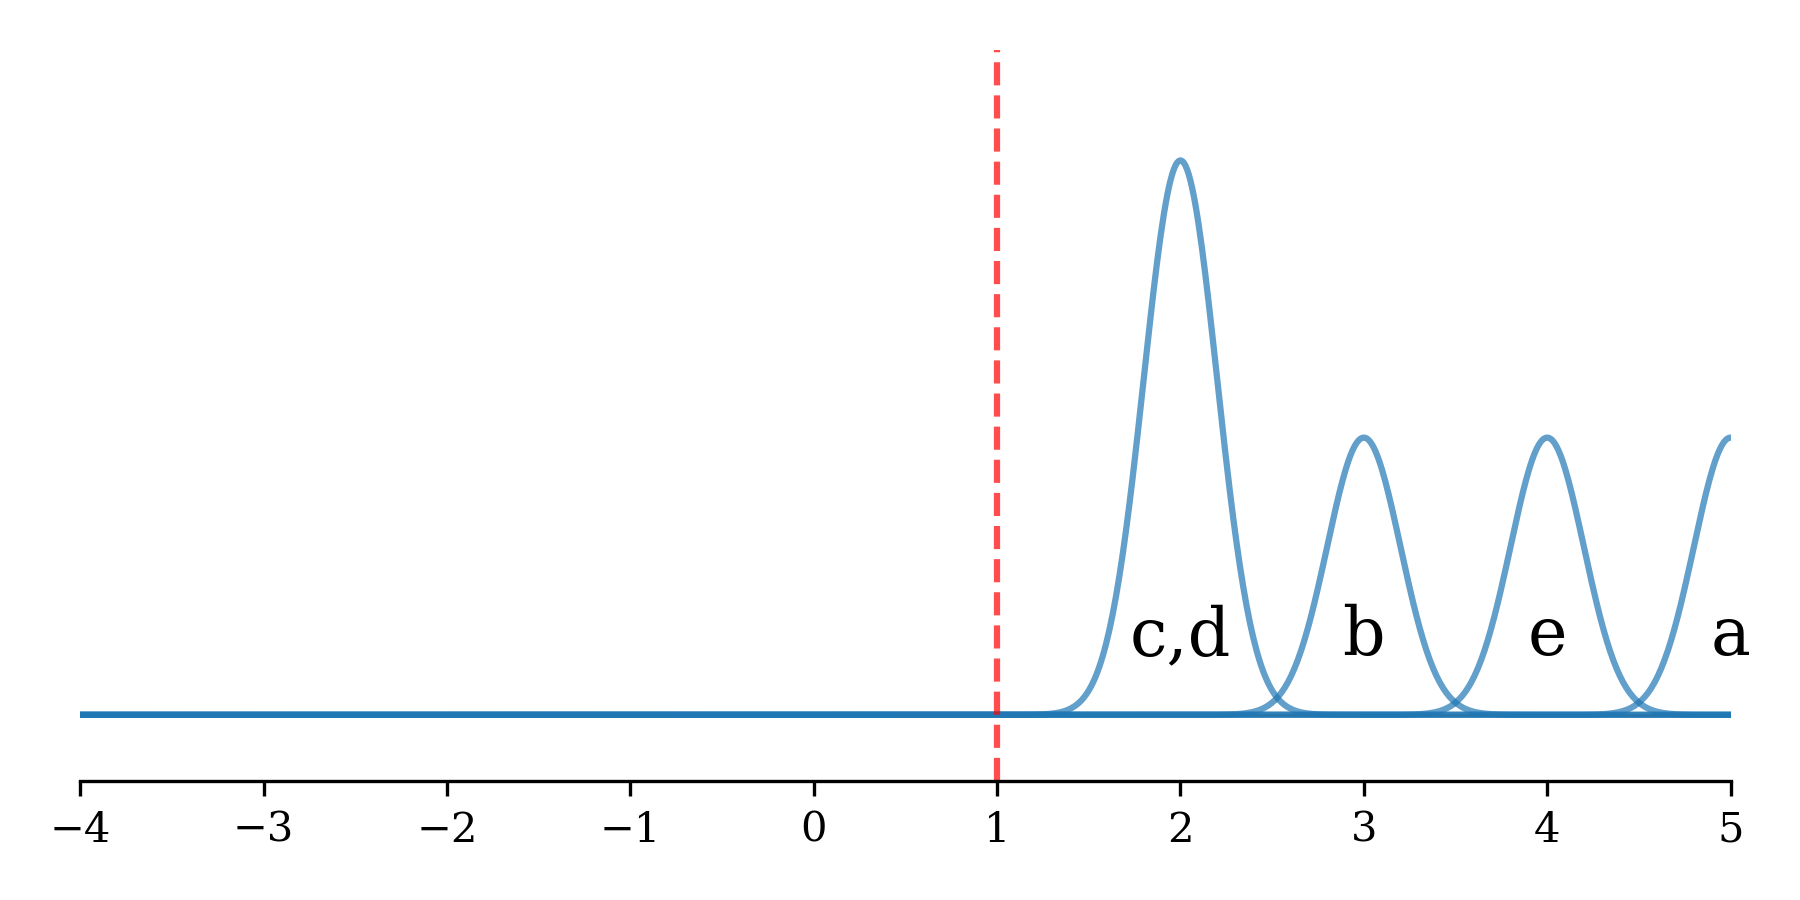
\includegraphics[width=\textwidth]{images/offset_abs_pos}
        \caption{Abs Positive Offset}
        \label{fig:abs_offset_up}
    \end{subfigure}

    \caption{Effects of decision boundary offsets on feature representation. The top row shows negative offsets and the bottom row shows positive offsets for both ReLU and Abs activated nodes.}
    \label{fig:offset_demo}
\end{figure}

Figure~\ref{fig:offset_demo} illustrates how offset perturbations affect feature selection for both ReLU and absolute value activation functions. With ReLU, offset perturbations modify the set of accepted features. The negative offset (Figure~\ref{fig:offset_demo}\subref{fig:relu_offset_down}) removes feature $c$ from the accepted set, leaving only $\{a, b\}$, while, with this distribution, a positive offset doesn't result in a chage (Figure~\ref{fig:offset_demo}\subref{fig:relu_offset_up}). 

In contrast, absolute value activation selects a single feature. A negative offset shifts the selection to feature $b$ instead of the originally trained feature $c$ (Figure~\ref{fig:offset_demo}\subref{fig:abs_offset_down}). A positive offset results in features $\{c, d\}$ having the minimum values (Figure~\ref{fig:offset_demo}\subref{fig:abs_offset_up}). However, neither of these aligns with the decision boundary, effectively resulting in an empty set.

These complete shifts in feature selection for the absolute value activation, compared to the incremental changes with ReLU, explain the more dramatic performance impact observed in Figure~\ref{fig:perturbation_analysis}, even with small offset perturbations.

\subsection{Scale Perturbations}

Analyzing the impact of scaling on intensity features presents a challenge due to the lack of a precise definition for what constitutes an intensity feature. Our experiments demonstrated that scaling activations, which directly modifies their magnitude, did not significantly affect the performance of either ReLU or absolute value networks. This invariance is unexpected if we assume that larger activations simply indicate stronger feature presence.

One possible explanation for this invariance could be the normalization effect of the LogSoftmax operation within the cross-entropy loss function. By renormalizing the output values, LogSoftmax might mitigate the impact of scaling on the relative differences between activations, potentially masking any effects on intensity-based features. However, this does not explain the performance drop observed when activations are scaled down to the magnitudes associated with distance features, suggesting a complex interplay between scaling and the different types of learned features.

\subsection{Cutoff Perturbations}

To further investigate intensity features, we introduced a threshold cutoff perturbation. This perturbation directly targets the ability to distinguish between features based on activation magnitude by clipping activations at a certain threshold. Our results showed a minor performance degradation for cutoff thresholds up to the 50th percentile, followed by a more moderate degradation as the threshold is further reduced. This suggests that the ability to distinguish between features with very high activations might not be critical for classification, especially if subsequent layers utilize sets of features rather than relying on individual activations, as indicated by our analysis of ReLU networks.

While the results of our intensity perturbation experiments generally support our hypothesis that neural networks prioritize distance-based features, the evidence is not as conclusive as with the distance perturbation experiments. Further investigation is needed to fully understand the role of intensity features and their interaction with different activation functions and network architectures.

\subsection{The Problem with Intensity}

Our perturbation analysis appears to support distance-based feature interpretation, but we must address a significant challenge: we cannot definitively disprove intensity-based interpretations due to the lack of a widely accepted definition of what constitutes an intensity feature. This ambiguity has persisted despite decades of research, with various interpretations proposed but no consensus reached. Some studies suggest that intensity features are indicated by maximum activation values, as seen in the foundational work on artificial neurons and perceptrons. Others propose that intensity features might be defined by activation values falling within a specific range, aligning with the concept of confidence intervals or thresholds.

The absence of a clear mathematical foundation for intensity metrics further complicates the matter. Distance metrics like Euclidean and Mahalanobis distances have well-defined statistical measures with clear linear formulations. However, we find no equivalent statistical measure for intensity that can be expressed through a linear equation. This lack of a concrete mathematical basis makes it challenging to design experiments that definitively target and assess intensity features.

Our scaling experiments highlight this difficulty. One might expect that doubling a strong signal (high activation) should make it stronger, yet our networks maintain consistent behavior under scaling. If we propose that relative values between nodes preserve intensity information, this begins to sound suspiciously like a distance metric.

The distance features in the network are easily explained as a Mahalanobis distance of a principal component as described in \cite{oursland2024interpreting}. But what is the statistical meaning behind the intensity features? It implies a complement to the principal component, a principal disponent consisting of an antivector, antivalue and an unmean. I don't think that principal disponents are real. What looks like an intensity metric is really a distance metric that matches everything except the large value. Perhaps statistical network interpretation has stymied researchers because we have been looking for the mathematical equivalent of Big Foot or the Loch Ness Monster.